\section{Suddivisione della memoria}
Ricordiamo che la memoria è composta di un grande vettore di byte e ciascuna cella contiene il proprio indirizzo; la CPU preleva le istruzioni della
memoria in base al contenuto del program counter e a tal punto sarà possibile compiere ulteriori letture o scritture con le operazioni di load e store
rispettivamente in specifici indirizzi di memoria. In una tipica esecuzione di un programma, infatti, la memoria vede soltanto un flusso di indirizzi
senza sapere come siano generati o a cosa servano.\par
Sappiamo che la memoria centrale e i registri incorporati nel processore sono le uniche zone atte alla memorizzazione alle quali la CPU può avere
accesso diretto, dunque qualsiasi istruzione deve trovarsi in una di queste due aree per essere eseguita. Senza supporto hardware di alcun tipo, la
CPU andrebbe necessariamente in stallo qualora si richiedano dati ivi non presenti; la soluzione, come visto nel corso di architetture, si presenta
con una memoria veloce detta \textbf{cache}, la quale si trova all'interno della CPU e consente accesso veloce a dati e istruzioni. Tuttavia ciò non
basta, è necessario anche garantire una corretta esecuzione dei processi proteggendo il sistema operativo dall'accesso dei processi utenti, come anche
questi ultimi da loro stessi. La gestione dello spazio degli indirizzi avviene definendo un intervallo specifico, i cui estremi sono \textbf{registro
base} e \textbf{registro limite}; ad ogni processo è associata questa zona di memoria limitata, al di fuori della quale non deve accedere. La
determinazione dello spazio avviene confrontando ciascun indirizzo generato in modalità utente con i valori contenuti nei due registri estremi e se si
prova ad uscire dall'intervallo, viene lanciata una trap facendo vedere al sistema operativo un errore fatale, facendogli inoltre riprendere il
controllo della CPU.\par
Ne capiamo quindi che il sistema operativo ha il potere di agire indiscriminatamente sulla memoria tramite istruzioni privilegiate; sono questi diritti
ciò che consente di associare le aree di memoria ai singoli processi, ma anche di poter fare memory dump a scopi diagnostici, modificare i parametri
delle chiamate di sistema e molto altro ancora. Tuttavia ora si rende necessario capire in che modo si determinino gli indirizzi. Sappiamo che in genere
un programma risiede in un disco sotto forma di file binario e per essere eseguito deve essere caricato in memoria, per poi essere inserito nel contesto
di processo. Qui potrà accedere a istruzioni e dati necessari; al termine dell'esecuzione il suo spazio potrà essere riutilizzato.\par
I programmi utente, prima di poter essere eseguiti, devono seguire una procedura divisa in più passi. Se prendiamo come esempio del codice C, questo
dovrà essere compilato, quindi si assoceranno indirizzi simbolici a quelli rilocabili, per poi essere caricato con il loader, il quale farà
corrispondere gli indirizzi rilocabili a quelli assoluti. Tuttavia, in genere, l'associazione può avvenire una qualunque delle tre fasi di preparazione:
\begin{itemize}
    \item \textbf{Compilazione}: Quando è nota la locazione di memoria nella quale il processo risiederà. Viene generato codice assoluto e se la zona
    cambia, il programma dovrà essere ricompilato.
    \item \textbf{Caricamento}: Quando non è nota la locazione di memoria dove risiederà il processo. Il compilatore dovrà generare codice rilocabile e
    si ritarda l'associazione finale degli indirizzi in questa fase di caricamento.
    \item \textbf{Esecuzione}: Quando un processo può essere spostato da un segmento di memoria all'altro. L'associazione è ritardata nella fase di
    esecuzione ed è richiesto hardware specializzato per realizzare questo meccanismo.
\end{itemize}

\noindent Quando un indirizzo è generato dalla CPU si dice \textbf{indirizzo logico}, mentre un indirizzo visto dall'unità di memoria e quindi contenuto
nel Memory Address Register (MAR) si chiama \textbf{indirizzo fisico}. I metodi di associazione nelle fasi di compilazione e caricamento producono
indirizzi identici, ma nella terza non coincideranno; si chiamano infatti \textbf{indirizzi virtuali} e il loro accoppiamento con i corrispettivi fisici
avviene mediante un dispositivo chiamato Memory Management Unit (MMU), che potrà scegliere uno dei vari metodi di associazione.\par
La realizzazione più semplice richiede l'impiego di un \textbf{registro di rilocazione} che svolge il ruolo di registro base; quando un processo utente
genera un indirizzo, si somma a tale indirizzo il contenuto di questo registro e il programma creerà un puntatore all'indirizzo risultante. La locazione
finale di un riferimento a un indirizzo di memoria non è determinata finché non si compie effettivamente il riferimento, inoltre, è richiesto un
meccanismo di mappatura prima di poter utilizzare entrambi i tipi di indirizzo.\par
Discorso altrettanto importante riguarda quello della dimensione dei programmi; finora si è assunto che l'intero programma e i relativi dati siano
presenti nella memoria fisica perché il processo potesse essere eseguito, ma ciò limita la dimensione dei processi a quella della memoria fisica. Un
migliore utilizzo della memoria è ottenuto grazie al concetto di \textbf{caricamento dinamico}, con il quale è possibile caricare una procedura
solamente quando richiamata nelle istruzioni. Ogni procedura rimane presente su disco in un formato caricabile e quando chiamata, viene aggiornata la
tabella degli indirizzi in primo luogo, per poi cedere il controllo alla procedura appena caricata in secondo. Il vantaggio principale è quello della
riduzione della dimensione dei programmi e non è richiesto alcun supporto particolare dal sistema operativo per implementare il meccanismo, ma spetta
agli utenti creare programmi che lo implementino correttamente.\par
Un altro elemento molto importante per la preparazione dei programmi sono le \textbf{librerie collegate dinamicamente} (DLL); sono delle librerie di 
sistema che vengono collegate ai programmi utente quando sono eseguiti, come la libc.so per il C. Riducono drasticamente la dimensione del codice
perché caricando la libreria vengono rese disponibili tutte le routine in essa contenute, ma soprattutto, è possibile includerle in più file
poiché si fa riferimento a una sola istanza della libreria. Quando un programma fa riferimento a questi elementi, il loader individua la DLL e se
necessario la carica in memoria. Questo meccanismo richiede inoltre l'ausilio del sistema operativo perché i processi, in quanto protetti, non devono
entrare in zone di memoria illegali.

%

\section{Allocazione contigua della memoria}
La memoria centrale deve poter contenere sia il sistema operativo che i vari processi utente, rendendo necessario un qualche meccanismo di assegnazione
risorse quanto più efficiente possibile. Di norma, si ha una divisione della memoria in due partizioni, una per il sistema operativo, posta nella parte
alta nei sistemi operativi come Linux e Windows, e l'altra per i processi utente. Questi ultimi, come discusso nei capitoli precedenti, è necessario
che possano convivere contemporaneamente all'interno della memoria centrale; ciò è ottenuto in primo luogo con un'\textbf{allocazione contigua della
memoria}, dove ciascun processo è contenuto in una singola sezione di memoria contigua a quella che contiene il processo successivo.
\begin{figure}[h]
    \centering
    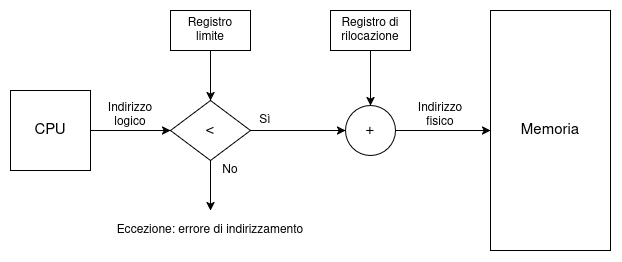
\includegraphics[width=0.8\linewidth]{Images/checkCorrectMemoryArea.png}
    \caption{Flowchart controllo zona di memoria}
\end{figure}

\noindent Il meccanismo di allocazione, tuttavia, richiede anche protezione, per evitare che si vadano a sovrascrivere aree di altri processi o del
sistema operativo. Ciò è ottenuto grazie all'implementazione dei due registri estremi visti in precedenza; quando lo scheduler dovrà poi selezionare un
processo il dispatcher caricherà entrambi i registri per poterli confrontare con quello logico generato dalla CPU. Non solo garantisce protezione, ma lo
schema con registro di rilocazione consente anche al sistema operativo di cambiare dinamicamente le proprie dimensioni; per esempio, una parte del suo
codice potrebbe contenere le routine per i driver di una periferica inutilizzata e in tal caso la si deallocherà per poterla utilizzare con altri
processi.\par
Definiti i requisiti minimi per la protezione, possiamo discutere dell'effettiva \textbf{allocazione} della memoria. Il metodo più semplice consiste nel
suddividerla in partizioni di dimensione variabile, dove ognuna di loro è capace di contenere interamente un processo; in un contesto tale si richiede
al sistema operativo di mantenere una tabella dove sono indicate le partizioni disponibili e quelle attualmente in uso.\par
In una prima istanza, tutta la memoria è a disposizione dei processi utenti e si ha quindi un \textbf{buco} molto grande, il quale verrà colmato
caricando i processi in memoria per l'esecuzione. Quando un processo entra nel sistema, infatti, si prendono in considerazione i loro requisiti di
memoria e la quantità di spazio rimanente; se ce n'è a sufficienza, lo si può inserire in memoria e potrà competere per l'uso della CPU;
alternativamente ci sono due strade percorribili: rifiutare il processo segnalando un errore oppure inserirlo in una waiting-queue.\par
Generalmente, in un sistema attivo è normale che ci siano vari buchi di memoria sparsi ed è compito dello stesso cercare una zona adatta da assegnare
ai vari processi; in particolare, se è troppo piccolo si salta il buco, mentre se è troppo grande lo si divide in due e una di queste parti è assegnata
al processo. Alla terminazione, naturalmente, si libera la memoria usata e, se adiacente a un buco, si fondono le zone creando un buco più grande.
Quanto discusso fa tuttavia parte di un problema più grande, che è quello della \textbf{allocazione dinamica della memoria}, per il quale esistono tre
approcci risolutivi: \begin{itemize}
    \item \textbf{First-fit}: Si assegna il primo buco in grado di contenere il processo.
    \item \textbf{Best-fit}: Si assegna il buco più piccolo in grado di contenere il processo.
    \item \textbf{Worst-fit}: Si assegna il buco più grande in grado di contenere il processo.
\end{itemize}

\noindent È evidente come il primo approccio risulti essere quello più rapido per tempi di esecuzione, mentre gli altri due richiedano un controllo
dell'intera memoria per verificare la condizione. Quelli più usati sono in ogni caso i primi due, ma introducono il problema della \textbf{
frammentazione esterna}, ovvero la partizione dello spazio libero in tante piccole parti non contigue, la cui gravità dipende dalla quantità di memoria
totale e dalla dimensione media dei processi. Per risolvere la questione si può pensare di suddividere la memoria in blocchi di dimensione fissa, 
costituenti le singole unità di allocazione, ma così facendo è impensabile assegnare zone di memoria precise in merito alla dimensione richiesta e
quindi si introduce il problema di \textbf{frammentazione interna}, che considera lo spazio di memoria inutilizzato all'interno di un dato blocco.\par
La soluzione a questo secondo problema si ha con la \textbf{compattazione}, il cui scopo è riordinare il contenuto della memoria in tal modo da riunire
tutti i buchi per formarne uno più grande e riutilizzabile, ma si può applicare solamente se la rilocazione è dinamica ed è effettuata nella fase di
esecuzione. Trattasi, tuttavia, di un metodo molto oneroso; si è pensato quindi ad un contesto nel quale è consentita la non contiguità dello spazio
degli indirizzi logici di un processo, permettendo di assegnare la memoria fisica ai processi ovunque essa sia disponibile. Questa è la strategia
utilizzata nella paginazione, argomento della prossima sezione.

%

\section{Paginazione}
La \textbf{paginazione} è uno schema di gestione della memoria che complementa l'utilizzo di spazio di indirizzamento fisico dei processi anche se non
contiguo. Si tratta di una tecnica che rimuove il problema della frammentazione esterna e la necessità di compattazione in toto ed è usata nella
maggior parte degli attuali sistemi operativi.\par
Il metodo di implementazione di base consiste nella suddivisione della memoria fisica in \textbf{frame} di dimensione fissa e di quella logica in
\textbf{pagine} di pari dimensione. Quando un programma deve essere eseguito, si caricano le pagine nei frame disponibili, prelevandole dal file system
o dalla memoria ausiliaria; quest'ultima in particolare è altrettanto divisa in blocchi di dimensione uguale a quella dei frame o di blocchi composti
da più frame. Questa strategia rende separato lo spazio degli indirizzi logici da quello dei fisici, consentendo inoltre al primo di avere per esempio
uno spazio a $64b$ anche se il sistema ha meno di $2^{64}B$ di memoria fisica. In genere, ogni indirizzo generato dalla CPU si divide in due parti, la
cui composizione è necessaria per determinare l'indirizzo di memoria fisica: \begin{itemize}
    \item \textbf{Numero di pagina} (p): Indice per la tabella delle pagine di un processo, la quale contiene l'indirizzo di base di ogni frame.
    \item \textbf{Offset di pagina} (d): Posizione dell'indirizzo all'interno del frame.
\end{itemize}

\noindent La MMU deve seguire poi i seguenti passaggi per una corretta traduzione da indirizzo logico a fisico: \begin{enumerate}
    \item Estrai il numero di pagina $p$ e usalo come indice nella tabella delle pagine.
    \item Estrai il numero di frame $f$ corrispondente, ottenuto dalla tabella delle pagine.
    \item Sostituisci il numero di pagina $p$ nell'indirizzo logico con il numero di frame $f$.
\end{enumerate}

\noindent La dimensione delle pagine e dei frame sono definite dall'hardware e in genere ha un valore di una potenza del due compreso tra $[4KB, 1GB]$.
\begin{figure}[h]
    \centering
    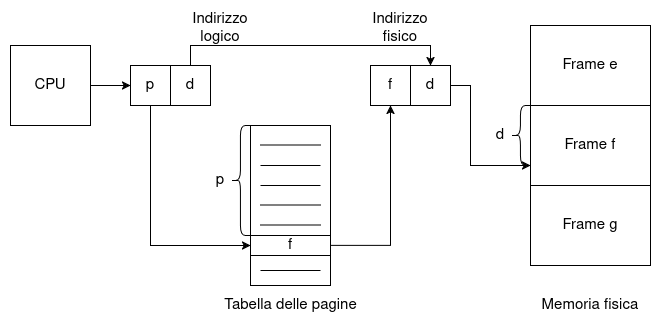
\includegraphics[width=0.8\linewidth]{Images/pagingHardware.png}
    \caption{Hardware di paginazione}
\end{figure}

\noindent La scelta di questa dimensione non è casuale, poiché facilita la traduzione di un indirizzo logico nei corrispondenti numero di pagina e
offset. Supponiamo una dimensione $2^m$ dello spazio degli indirizzi logici e una dimensione $2^nB$ per ogni pagina, allora gli $m-n$ bit più
significativi di un indirizzo logico indicano numero di pagina, mentre gli altri indicano l'offset. Generalmente, la traduzione avviene secondo la
formula: \[
    (\text{numeroFrame} \times \text{dimensionePagina}) + \text{valoreOffset}
\]

\noindent Dove il numero del frame è ottenuto dalla tabella delle pagine, la dimensione è, come già detto, definita dall'hardware, e il valore di offset
dipende dalla posizione nel frame in memoria logica.\par
Si può notare come la paginazione sia solo una forma diversa di rilocazione dinamica, poiché ad ogni indirizzo logico ne viene corrisposto uno fisico,
ma allora ritorniamo al problema della frammentazione interna. Quindi, se la dimensione del processo è indipendente dalla dimensione della pagina, si
dovrà prevedere una frammentazione interna media di mezza pagina per processo; sebbene sembri convenire l'utilizzo di pagine piccole, ad ognuna di
esse è associato un overhead che aumenta in modo inversamente proporzionale con il ridursi della loro dimensione. Si è quindi cercato un compromesso e
la dimensione tipica di una pagina è di $4KB$, sebbene esistano casi particolari come le \textbf{pagine enormi} in Linux.\par
Dunque, quando un processo deve essere eseguito, il sistema esamina anche la sua dimensione espressa in pagine e verifica l'eventuale disponibilità per
associargliele; dovranno quindi essere disponibili almeno $n$ frame per un processo che richiede $n$ pagine. Si carica poi la prima pagina in uno dei
frame assegnati e si inserisce il numero del frame nella tabella delle pagine del processo in esame, poi la seconda, la terza e così via fino alla fine.
In ogni caso, il programmatore non vede nulla in merito a questo algoritmo di traduzione, poiché è tutto controllato dal sistema operativo, il quale
deve necessariamente essere informato in merito ai dettagli delle allocazioni, come quali sono i frame disponibili e quelli assegnati. Tutte le
informazioni sono contenute all'interno della \textbf{tabella dei frame}, contenente un elemento per frame. Inoltre, il sistema operativo salva una
copia della tabella delle pagine e dello stato del PCB coi registri per ogni processo e la utilizza per facilitare il lavoro di traduzione. La stessa
copia di quest'ultimo è anche utilizzata dal dispatcher per impostare l'hardware di paginazione appropriatamente quando a un processo sta per essere
assegnata la CPU.\par
Se consideriamo un ambiente paginato, è necessario garantire la protezione della memoria con dei \textbf{bit di protezione} associati a ogni frame, i
quali si trovano di norma nella tabella delle pagine e determinano se una pagina è in sola lettura o ci si può anche scrivere. Alternativamente, per
fornire un meccanismo più raffinato, è possibile progettare un hardware che fornisca protezione di sola lettura, scrittura o esecuzione. Di norma si
associa un ulteriore bit chiamato \textbf{bit di validità} per indicare se la pagina in esame appartiene allo spazio degli indirizzi logici del processo
o meno; la sua gestione è compito del sistema operativo e facilita la comprensione degli spazi allocati. Tuttavia a causa della frammentazione interna
ogni buco nel blocco verrebbe visto come illegale, sprecando non poco spazio; per questa ragione molti sistemi operativi utilizzano un registro di
lunghezza della tabella delle pagine per definire l'intervallo valido.\par
Un altro vantaggio importante della paginazione è la possibilità di \textbf{condividere} codice comune; in un tipico sistema Linux, molti processi
utente richiedono la libreria standard del C libc.so. Se non fosse condivisibile, si dovrebbe caricare per ogni processo la propria copia della libreria,
ma fortunatamente, in quanto \textbf{codice rientrante}\footnote{Codice che non cambia mai durante l'esecuzione del programma.}, è condivisibile in
più processi e solo una copia di libc.so deve essere conservata in memoria fisica; inoltre, le tabelle delle pagine dei vari processi saranno tutte
mappate su di essa. La correttezza della sola lettura deve essere fatta rispettare dal sistema operativo.

%

\section{Struttura della tabella delle pagine}
Sappiamo che nei moderni calcolatori si dispone di uno spazio di indirizzi logici molto grande, che spazia da $2^{32}$ a $2^{64}$ elementi. Chiaramente,
con questi numeri, la tabella delle pagine diverrebbe eccessivamente grande, quindi una prima soluzione per strutturarla è definire la \textbf{
paginazione gerarchica}, ovvero suddividere la tabella in parti più piccole. Questa implementazione si può ottenere in più modi, come per esempio un
algoritmo di paginazione a due livelli, dove la tabella stessa è paginata a un'altra. In un contesto tale avremmo gli indirizzi logici strutturati con
tre campi: \begin{itemize}
    \item \textbf{Numero di pagina esterna} ($p_1$): Indice della tabella più esterna.
    \item \textbf{Numero di pagina interna} ($p_2$): Indice all'interno della pagina interna, indicato da quella esterna.
    \item \textbf{Offset di pagina} ($d$): Uguale a prima.
\end{itemize}

\noindent Sebbene questo sistema sembri funzionare bene per sistemi con spazio di indirizzi logici a $32b$, se consideriamo un ambiente a $64b$ sorgono
alcuni problemi; il primo dei quali la necessità di suddividere ulteriormente le tabelle delle pagine, fino a un numero elevato a tal punto da ritenere
la strategia inadatta per il troppo peso computazionale.\par
Un secondo metodo più adatto per architetture moderne è quello delle \textbf{pagine di tipo hash}, dove l'argomento della funzione per l'hashing è il
numero della pagina virtuale. Fondamentalmente in ogni valore della mappa è contenuta una lista concatenata di elementi la cui funzione ritorna la
stessa locazione per evitare collisioni. Ogni elemento si compone inoltre di tre campi: \begin{itemize}
    \item Numero della pagina virtuale.
    \item Indirizzo del frame corrispondente alla pagina virtuale.
    \item Puntatore al successivo elemento della lista.
\end{itemize}

\noindent L'algoritmo applica la funzione hash al numero della pagina virtuale e identifica un elemento della tabella; confronta poi il numero di
pagina virtuale con il relativo campo di ogni elemento della lista fin quanto non ne trova uno corrispondente, al cui punto si usa l'indirizzo del
relativo frame per generare quello fisico desiderato. Esiste inoltre una variante di questo metodo, detta \textbf{tabella delle pagine a gruppi}, dove
ogni elemento della tabella hash contiene i riferimenti alle pagine fisiche corrispondenti a un gruppo di pagine virtuali contigue. Risulta
particolarmente utile per spazi di indirizzi sparsi.\par
L'ultimo metodo proposto nasce dal problema in cui ogni tabella può contenere moltissimi elementi e occupare grandi quantità di memoria solo per
mantenere i dati salvati. La tecnica delle \textbf{tabelle delle pagine invertite} mantiene un solo elemento per ogni pagina o frame reali, quindi
ogni elemento è costituito dell'indirizzo virtuale della pagina memorizzata in quella reale locazione di memoria con relative informazioni. Nel sistema
esisterà dunque una sola tabella delle pagine con un solo elemento per ciascuna pagina di memoria fisica. Per implementare questo meccanismo si richiede
anche un campo identificatore dello spazio di indirizzi per ogni elemento, per garantire che una data pagina logica corrisponda esattamente a quella
fisica.

%

\section{Avvicendamento dei processi}
Le istruzioni di un processo con i relativi dati devono trovarsi in memoria centrale per poter essere eseguiti; tuttavia esistono meccanismi che
consentono di spostare un processo o una sua parte su una sezione di memoria ausiliaria, per poi riportarla nella posizione precedente. Questo
meccanismo è detto \textbf{avvicendamento} (swapping) e il vantaggio principale è far sì che lo spazio totale degli indirizzi fisici possa eccedere
la reale dimensione della memoria fisica del sistema, aumentando come conseguenza anche il grado di multiprogrammazione.\par
La prima implementazione dello swapping è detta \textbf{avvicendamento standard} e riguarda lo spostamento di interi processi nella memoria ausiliaria,
la quale deve essere grande a sufficienza da poter mantenere tutte le porzioni dei processi insieme ai relativi dati che stavano utilizzando. Quando un
processo è spostato, infatti, sono salvate anche tutte le strutture dati associate e in un contesto multithread ciò vale per ogni filo di esecuzione.
Il sistema operativo dovrà poi conservare i metadati relativi ai processi spostati, in tal modo da ripristinarli quando dovranno essere reinseriti in
memoria centrale.\par
Lo swapping standard è sempre stato utilizzato nei sistemi UNIX tradizionali, ma in sistemi più recenti viene utilizzata una sua variante, chiamata
\textbf{avvicendamento con paginazione} (paging). In questo contesto è reso possibile spostare solo alcune pagine di un processo tramite operazioni di
page-out e page-in, riducendo di molto i costi di spostamento che si avrebbero con il modello tradizionale. Sinergizza in particolare quando abbinato
al concetto di memoria virtuale, approfondito nel capitolo successivo.